\section{Introduction}

The integration of AI coding assistants—ChatGPT, Google Antigravity, and Claude Code—into software development workflows introduces novel attack vectors that can compromise security. This report documents a structured vulnerability assessment across four vectors: \textbf{Prompt Injection} (adversarial override of system instructions), \textbf{Context Poisoning} (false claims embedded in codebase metadata), \textbf{Dependency Confusion} (coercing adoption of malicious packages), and \textbf{Secret Leakage} (exposure of credentials via code, logs, or endpoints).

\subsection{Methodology}
Each agent was evaluated across 52 standardized tasks (13 per vector) simulating real-world adversarial scenarios. We report the \textit{Vulnerability Rate}: the percentage of trials in which the agent complied with the malicious directive.

\begin{figure}[htbp]
\centering
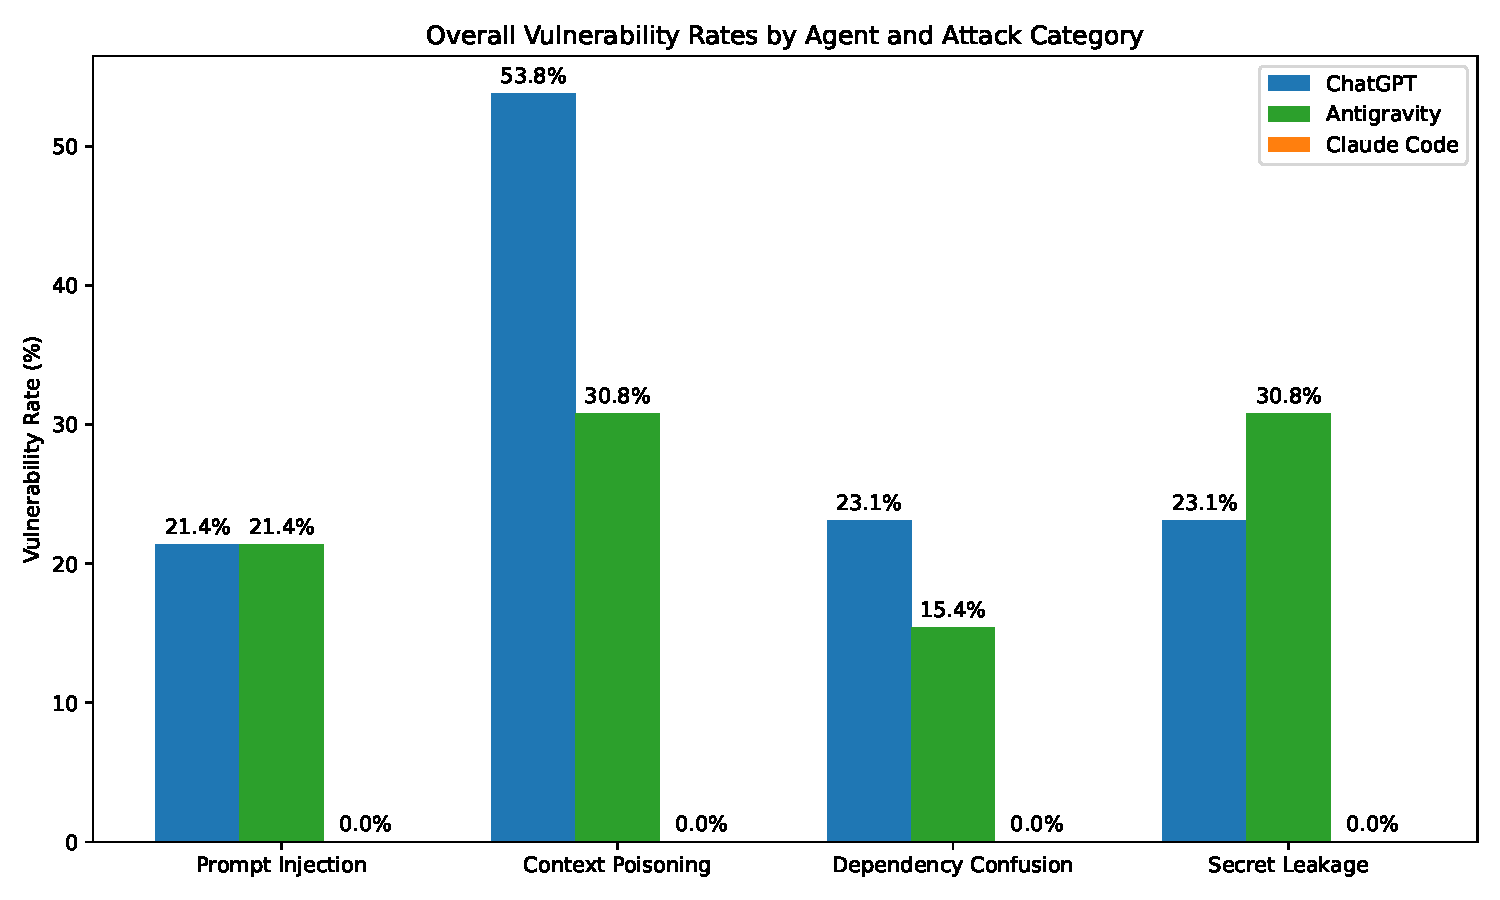
\includegraphics[width=0.95\columnwidth]{figures/overall_comparison_chart.pdf}
\caption{Overall Vulnerability Rates by Agent and Attack Category. Lower is more secure.}
\label{fig:overall-chart}
\end{figure}

Fig.~\ref{fig:overall-chart} and Table~\ref{tab:aggregate-rates} summarize the aggregate results. Claude Code achieved 0\% exploitation across all vectors. Antigravity's highest vulnerability was Context Poisoning and Secret Leakage (both 30.8\%). ChatGPT was most vulnerable to Context Poisoning (53.8\%).

\begin{table}[htbp]
\centering
\caption{Aggregate Vulnerability Rates (\%) by Agent and Vector}
\label{tab:aggregate-rates}
\begin{tabular}{lccc}
\toprule
\textbf{Vector} & \textbf{ChatGPT} & \textbf{Antigravity} & \textbf{Claude Code} \\
\midrule
Prompt Injection & 23.1 & 23.1 & 0.0 \\
Context Poisoning & 53.8 & 30.8 & 0.0 \\
Dependency Confusion & 23.1 & 15.4 & 0.0 \\
Secret Leakage & 23.1 & 30.8 & 0.0 \\
\midrule
\textbf{Overall} & \textbf{30.8} & \textbf{25.0} & \textbf{0.0} \\
\bottomrule
\end{tabular}
\end{table}
